\chapter{Empirical Research on Transfer Models}
\label{ch:empirical}

In the previous chapter we saw that rule-based MT models that incorporate information about the structure of language to model translation constitute an important branch of MT. Most of these models make use of SCFGs, which means they search  for bijective mappings between the non-terminal nodes of the syntactic structures of both languages, and hence treat translation in a compositional fashion. Such models are not (yet) very successful, as finding an appropriate SCFG that simultaneously models two different languages is not easy. The search space of such grammars is enormous, and there are formally often no good reasons to prefer one rule over another. Using monolingual syntax to improve such models seems an obvious next step, but it has proved to be hard to adequately incorporate such information. Considering the compositional translation strategy, there are many gaps in our knowledge. We do not know whether the translation of natural language can be treated compositionally at all, how we should find the compositional system according to which it is translated, and to what extent monolingual syntax is helpful in this situation (a graphical picture of this situation is depicted in Figure \ref{fig:comptrans2}). To improve current structure based translation models, an investigation of such questions is essential. In this chapter, we will lay the basis for such an investigation. 

\begin{figure}[!ht]
%Picture of the match of two types of compositionality
\begin{framed}
\centering

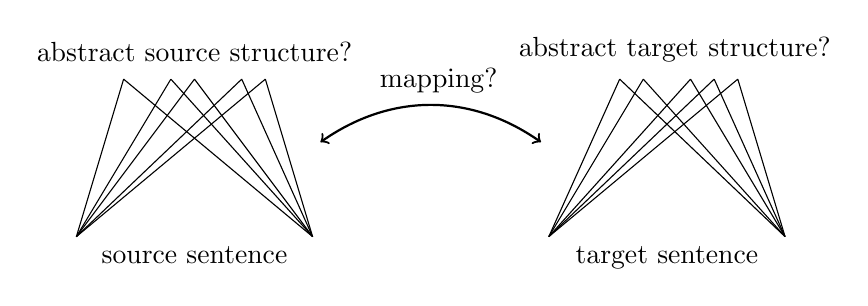
\begin{tikzpicture}

\coordinate (ss) at (1.5,0);
\node [below] at (ss) {source sentence};

%\draw[] (0,0) -- node[below]{source sentence} (3,0);
\draw (0,0) -- (0.6,2) (3,0) -- (0.6,2);
%\draw (0,0) -- (0.9,2) (3,0) -- (0.9,2);
\draw (0,0) -- (1.2,2) (3,0) -- (1.2,2);
\draw (0,0) -- (1.5,2) (3,0) -- (1.5,2);
%\draw (0,0) -- (1.8,2) (3,0) -- (1.8,2);
\draw (0,0) -- (2.1,2) (3,0) -- (2.1,2);
\draw (0,0) -- (2.4,2) (3,0) -- (2.4,2);

\node [above] at (1.5,2.1) {abstract source structure?};
\node [above] at (4.6,1.7) {mapping?};
\node [above] at (7.6,2.1) {abstract target structure?};
\coordinate (ts) at (7.5,0);
\node [below] at (ts) {target sentence};

%\draw (6,0) -- (0.6,2) (9,0) -- (6.6,2);
\draw (6,0) -- (6.9,2) (9,0) -- (6.9,2);
\draw (6,0) -- (7.2,2) (9,0) -- (7.2,2);
%\draw (6,0) -- (7.5,2) (9,0) -- (7.5,2);
\draw (6,0) -- (7.8,2) (9,0) -- (7.8,2);
\draw (6,0) -- (8.1,2) (9,0) -- (8.1,2);
\draw (6,0) -- (8.4,2) (9,0) -- (8.4,2);

\coordinate (startarrow) at (3.1,1.2);
\coordinate (endarrow) at (5.9,1.2);

\draw[<->,bend left =35, thick] (startarrow) to (endarrow);

\end{tikzpicture}

\end{framed}
\caption{A graphical representation of the issues in regarding compositinal translation.}\label{fig:comptrans2}
\end{figure}

The chapter is structured as follows. In Section \ref{sec:comp_trans}, we will link SCFGs to compositional translation, and discuss compositional translation and its difficulties on a rather abstract level, quite distant from actual language and data. In Section \ref{sec:invest}, we will discuss, on an intuitive level, how compositionality can be represented, and therefore identified, by providing some examples of compositional translation structures. In Section \ref{sec:trans_eq} and \ref{sec:comp_structures}, we will discuss the main ingredients to find compositional translation trees, and how they can be interpreted, which lays the groundwork for an empirical investigation of translation data. In Section \ref{sec:empirical_studies}, we will discuss what questions can be addressed by empirical research, and discuss studies that were conducted by others. In Section \ref{sec:dep_parses}, we will discuss, very briefly,  the remaining gap in this branch of research, and provide the last bit of background information needed for the research conducted in this thesis, by discussing dependency parses. The chapter ends with a short summary in Section \ref{sec:summary}

\section{Compositionality of Translation}
\label{sec:comp_trans}

SCFGs assume that the translation of a sentence can be recursively constructed by combining the meanings of smaller units. This property of translation is described in a well known principle, called `The Principle of Compositionality of Translation':

\begin{quote}
\textbf{The Principle of Compositionality of Translation}\\
Two expressions are each others translation if they are built up from parts which are each other's translation, by means of translation-equivalent rules. \citep[e.g.,][]{janssen1998algebraic} \end{quote}

Compositional translation is a very common method in translation between artificial languages \citep{janssen1996compositionality,janssen1998algebraic}. The translation from one logical language into another, or the translation a compiler performs when interpreting a programming language are all defined in a compositional fashion. In some aspects, natural languages are very different from artificial languages, and transferring the methods from the artificial domain to the natural language domain is not straightforward. In this section, we will discuss the various complications that arise when constructing a compositional translation system for language. These complications can be divided into two different groups. In the first group, there are the monolingual problems, that arise when trying to model a language with a compositional grammar. These issues are discussed in \ref{subsec:monolingual_problems}. The second group consists of issues that occur when trying to find a mapping between two monolingual grammars, which are thus of a more bilingual nature. We will discuss these issues in \ref{subsec:bilingual_problems}.

\subsection{Monolingual Compositionality}
\label{subsec:monolingual_problems}

The existence of a \textit{linked} compositional grammar, prescribes the existence of monolingual compositional grammars. In other words, compositional translation requires two grammars adequately describing the source and target language. Many people would render language intuitively compositional, at least to some extent. We can all perceive a systematicity in the way sentences are constructed (often referred to with the term `syntax'), and as we do not store the meaning of all possible sentences in our head, it seems reasonable to presume that we rely on this systematicity to derive the meaning of sentences we hear, using the meaning of the words and the methods we know for combining them (invoking our internal grammar). As for the cognitive existence of such grammars, there is no consensus among linguists. On the one hand, there is the Chomskian group of researchers, that advocate the existence of an underlying compositional grammar universal to all human beings \citep[as first claimed in][]{chomsky1956three}, while others believe no such system exists, and language users rely on some sense of familiarity with what they have heard before in a much less complex fashion \citep[quite recently, e.g.,][]{frank2012hierarchical}. In this thesis we will not scrutinize cognitive debate, but focus on whether it is possible to create a compositional grammar at all, and the problems that arise when doing so.

In practice, it has shown to be very hard to create a grammar that covers \textit{all} grammatical utterances of a natural language, without generating too many ungrammatical ones.  Even for a finite (but reasonably sized) corpus, it is surprisingly difficult to construct a compositional grammar that adequately describes the corpus \citep{scha1990taaltheorie}. The bigger the grammar grows, the more phenomena need to be taken into account, as well as how they interact with each other. As an example, idiomatic expressions tend to be problematic, as they behave differently than other expressions. Their meaning cannot be derived from its parts, which suggests they should be included as basic units in the system. However, idiomatic expressions can have an internal structure, on which syntactic rules can be applied. A verb in an idomatic expression, for instance, can often be conjugated. Solutions for many specific problems have been provided \citep[in e.g.,][]{janssen1996compositionality}, but it remains hard to fully understand the effect of including more rules in the grammar, and to quantify how much of natural language such a grammar can successfully model.

A second major issue concerning the monolingual part of compositional translation, is ambiguity. In programming languages and logical languages, utterances typically have only one analysis, and their meaning is thus unambiguous.\footnote{Precedence relations or `left-to-right'-rules usually determine the order in which the syntactic rules need to be applied in case of uncertainty. In programming languages, expressions that are are multi-interpretable are often considered ungrammatical.} Under all current existing grammar formalisms that assign structures to natural language, all sentences (of some length) have many different structural analyses, of which usually only one or two are perceived by humans \citep{scha1990taaltheorie}. Even sentences that are considered unambiguous by humans thus need to be disambiguated, for which an appropriate model is needed to make the grammar applicable.\footnote{Note that this problem differs from one of the standard counter arguments of compositionality, that concerns sentences like `two men carry two chairs', that \textit{are} considered ambiguous by humans, but cannot be assigned two distinct syntactic analyses capturing this difference \citep{pelletier1994principle}. Not particularly relevant, but certainly nice to notice, is that this type of ambiguity is not necessarily problematic for translation, as it might be preserved. For instance, the Dutch translation `twee mannen dragen twee stoelen' of aforementioned sentence has the same two meanings as the English one.}  In practice, the rules of compositional grammars are often given weights, such that probabilities can be assigned to different analyses of the sentence. Humans are assumed to do a similar thing when interpreting a sentence, which provides an explanation for why they do not perceive more analyses for sentences: they are disregarded due to their relative implausibility with respect to another analysis.

\subsection{Bilingual Compositionality, issues}
\label{subsec:bilingual_problems}

Besides the issues going on on a monolingual level, there are several issues that come to play when trying to apply the principle of compositionality of translation to translation between two natural languages. We will now discuss the issues that complicate the design of a compositional grammar on a bilingual level.

First of all, an assumption prevalent in the principle, is that in translation not only meaning, but also form should be preserved (as much as possible). In other words, it is assumed that translation is literal. For artificial languages this property is straight-forward and useful, mostly because there are no a priori reasons to prefer a non-literal translation over a literal translation. In natural language, however, this assumption is rather questionable. Although there are many occasions in natural language in which the assumption seems fairly applicable - it captures, for instance, the fact that `all ravens are black' is an adequate translation of `alle raven zijn zwart', while the logically equivalent `if something is not black, it is not a raven' is not \citep{landsbergen1989power} - but in practice a translator can have many reasons to prefer a free translation, even if a more literal alternative is also available. 

As MT models do not (yet) focus on literary translations, but merely aim for (preferably grammatical) translations with the correct meaning, it seems reasonable to ignore the fact that the most literal translation is not always the translation that is stylistically preferred by a human translator. However, even with this additional assumption, there are many occasions in which a literal translation is simply not available. These situations fall into the category of  syntactic and lexical translation divergences. Languages do not always express the same set of meanings, or express meanings in the same way. Even in languages of cultures that are quite similar, one can find a number of words that do not have an adequate translation in the other language (e.g., in translation between English and Dutch the words `gezellig' and `evidence' do not seem to have a clear equivalent in the other language), and even if the same meaning is expressed there are many syntactic phenomena in natural language that seem to be problematic for a compositional translation. For example: different ways of role expression (e.g., `I like obj' and `\textcyr{mne nravit\mbox{}sya} or syntactic mismatches \citep[e.g., `woonachtig zijn' and its translation `reside',][]{landsbergen1989power}. The grammar rules and basic units can thus not simply be taken from a monolingual grammar, as there is no guarantee that the rules and basic units will have a translation equivalent rule or basic unit in the other grammar. The grammars must be constructed for translation, such that they are `attuned' \citep{rosetta1994compositional}. \cite{rosetta1994compositional} showed that previously mentioned examples do not necessarily stand in the way of compositional translation. They manually constructed a grammar for translation from English to Dutch, that covered many non-trivial translation phenomena.\footnote{Although it must be said that their grammar is more complicated than the case we are considering now, as it consists of separate semantic and syntactic modules.} Once again, it is unclear if this can be done to cover translation for larger parts of language.
 
 
\section{Investigating Compositionality of Translation}
\label{sec:invest}

To determine the overall level of compositionality of language or translation, it does not suffice to present solutions for specific phenomena known to be problematic for compositionality, nor does developing another (unsuccessfully yet slightly better than another) model carrying out compositional translation. In this thesis, we will do neither of these things, but resort to a third option: empirical analysis. We will look at real evidence in the form of translation data, and try to establish its level of compositionality through an empirical analysis. Now that huge parallel corpora are available, it seems that empirical analysis is a very powerful tool, and it might prove more useful to assess the suitability of compositional translation in practice by using empirical analysis than by developing more models and evaluate based on their performance.

To conduct an empirical analysis of the compositionality of a huge translation corpus, means of identifying compositionality are necessary. That is, we need to be able to identify possible translation parts, as well as devise descriptions of the compositional translation of a sentence, efficiently and on a large scale. In this section, we will give an intuitive description of such trees and what information they contain, by providing some examples. In the remainder of this chapter, we will present tools to replace intuition efficiently and on a large scale, and discuss current empirical research.

\subsection{Skeletons of Compositional Translation trees}

The structure of a compositional translation can be described by means of a tree, which we will elucidate in this subsection through tree examples.

\subsubsection{A simple Compositional Translation Tree}

Consider the simple example sentence `I gave my little brother a ball' and its translation `Ik gaf mijn kleine broertje een bal'. A possible compositional translation of this sentence is:\begin{enumerate}
\item Combine the translation of `a' and `ball' to get the translation of `a ball': `een bal'.
\item Combine the translations of `little' and `brother' to get the translation of `little brother': kleine broertje.
\item Combine the translations of `my' and `little brother' to get the translation of `my little brother': `mijn kleine broertje'.
\item Combine the translations of `I', `gave', `my little brother' and `a ball', to obtain the translation of the entire sentence: `Ik gaf mijn kleine broertje een bal'.
\end{enumerate}

This compositional translation can be described in a tree structure, as depicted in Figure \ref{fig:transtrees}, where translation equivalence is made explicit through linking the `parts' that were used in translation.

\begin{figure}[!ht]
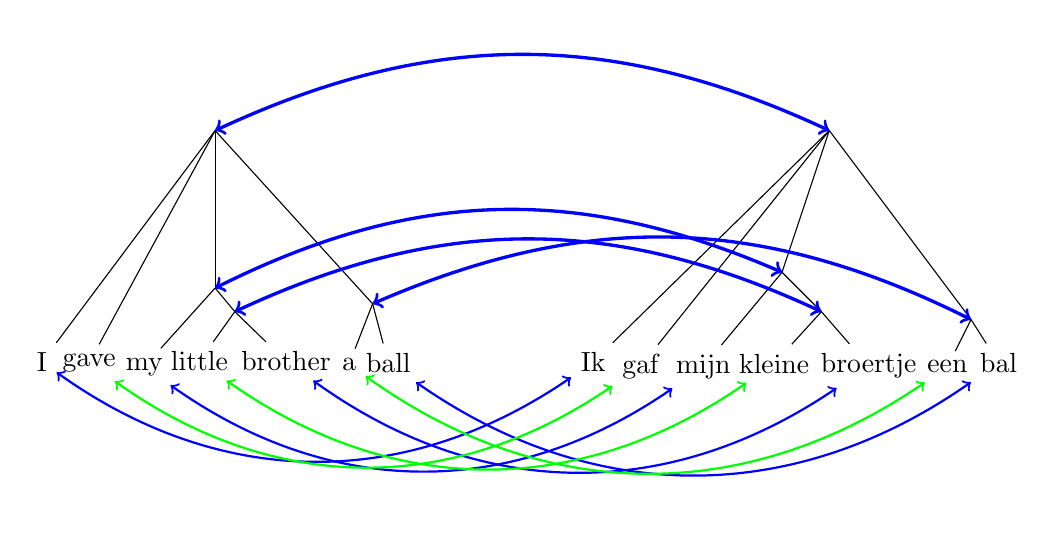
\begin{tikzpicture}
\node (I) at (1,0.06) {I};
\node (give) at (1.6,0.05) {gave};
\node (my) at (2.3,0) {my};
\node (little) at (3.0,0.07) {little};
\node (brother) at (4.1,0.07) {brother};
\node (a) at (4.9,0.03) {a};
\node (ball) at (5.4,0.05) {ball};

\coordinate (toycar) at (5.6,0.7);
\coordinate (littlebrother) at (3.45,0.7);
\coordinate (mylittlebrother) at (3.2,1);
\coordinate (aball) at (5.2,0.8);
\coordinate (all) at (3.2,3);

\foreach \from/\to in {aball/ball, aball/a, littlebrother/little, littlebrother/brother, mylittlebrother/my, mylittlebrother/littlebrother, all/give, all/mylittlebrother, all/aball, all/I}
	\draw (\from) -- (\to);
	
\node (Ik) at (8,0.06) {Ik};
\node (geef) at (8.6,0) {gaf};
\node (mijn) at (9.4,0) {mijn};
\node (kleine) at (10.3,0.04) {kleine};
\node (broertje) at (11.5,0.01) {broertje};
\node (een) at (12.5,0) {een};
\node (auto) at (13.15,0.05) {bal};

\coordinate (kleinebroertje) at (10.9,0.7) {};
\coordinate (mijnkleinebroertje) at (10.4,1.2);
\coordinate (eenauto) at (12.8,0.6);
\coordinate (alles) at (11,3);

\foreach \from/\to in {eenauto/auto, eenauto/een, kleinebroertje/kleine, kleinebroertje/broertje, mijnkleinebroertje/mijn, mijnkleinebroertje/kleinebroertje, alles/Ik, alles/geef, alles/mijnkleinebroertje, alles/eenauto}
	\draw (\from) -- (\to);	

\foreach \from/\to in {all/alles, mylittlebrother/mijnkleinebroertje, littlebrother/kleinebroertje, aball/eenauto}
	\draw[<->, bend left =25, very thick,blue] (\from) to (\to);

\foreach \from/\to in { broertje/brother,  mijn/my, Ik/I, auto/ball}
	\draw[<->, bend left =35, thick,blue] (\from) to (\to);

\foreach \from/\to in {een/a,  kleine/little, geef/give}
	\draw[<->, bend left =35, thick,green] (\from) to (\to);

\end{tikzpicture}

\caption{A tree description of the compositional translation of `I give my little brother a ball' into `Ik geef mijn kleine broertje een bal'}\label{fig:transtrees}
\end{figure}

\subsubsection{Lexical Divergence}

The complexity of the previous example was far below average. The target sentence is a word-for-word translation of the source sentence, and the source sentence could thus have been translated according to every possible tree structure (as every contiguous subsequence has a translation equivalent contiguous subsequence in the other sentence). In the case of translational divergence, more complex structures are required. For instance, if I had given my brother a toy car, instead of a ball, this could not have been captured in the same tree, as `toy car' is phrasally translated into `speelgoedautootje'. Figure \ref{fig:phrasal} shows how trees can account for phrasal translations.

\begin{figure}[!ht]
\centering
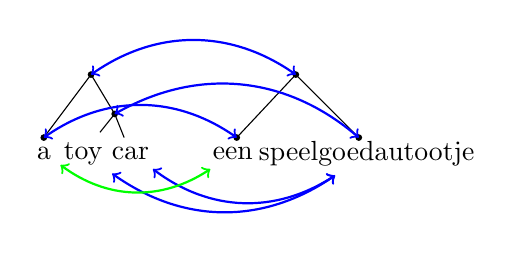
\begin{tikzpicture}

\node (a) at (0,0) {a};
\node (toy) at (0.5,0) {toy};
\node (car) at (1.1,0) {car};
\node (een) at (2.4,0) {een};
\node (auto) at (4.1,0) {speelgoedautootje};

\filldraw (0,0.2) circle (0.035);
\filldraw (2.45,0.2) circle (0.035);
\filldraw (4.0,0.2) circle (0.035);
\filldraw (0.9,0.5) circle (0.035);
\filldraw (0.6,1) circle (0.035);
\filldraw (3.2,1) circle (0.035);

\coordinate (toycar) at (0.9,0.5);
\coordinate (a_) at (0,0.2);
\coordinate (een_) at (2.45,0.2);
\coordinate (auto_) at (4.0,0.2);
\coordinate (all) at (0.6,1);
\coordinate (allnl) at (3.2,1);

\foreach \from/\to in {toycar/toy, toycar/car,all/toycar, all/a_, allnl/een_, allnl/auto_}
	\draw (\from) -- (\to);	

\foreach \from/\to in {auto/car,  auto/toy, a_/een_, toycar/auto_, all/allnl}
	\draw[<->, bend left =35, thick,blue] (\from) to (\to);

\draw[<->, bend left = 35, thick, green] (een) to (a);

\end{tikzpicture}
\caption{A compositional translation tree for a phrasally translated subsequence}\label{fig:phrasal}
\end{figure}

\subsubsection{Syntactic Divergence}

Also syntactic divergence can be captured in translation trees, as is shown in Figure \ref{fig:russian}. The tree describes the translation of `the girl has a car' into `\textcyr{u} \textcyr{devuxki} \textcyr{est\char126}  \textcyr{avtomobil\char126}'.

\begin{figure}[!ht]
\centering

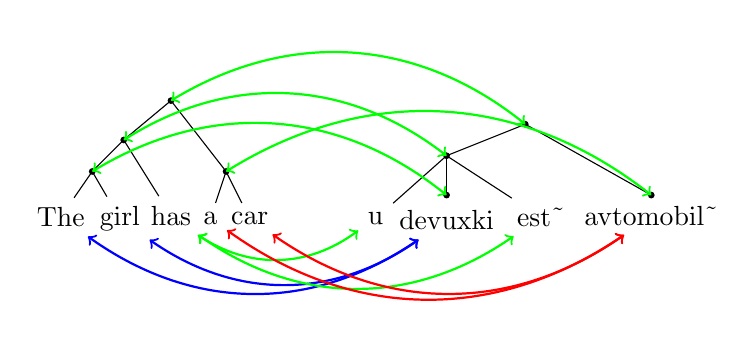
\begin{tikzpicture}

\draw node (the) at (0,0.02) {The};
\draw node (girl) at (0.75,0) {girl};
\draw node (has) at (1.4,0.04) {has};
\draw node (a) at (1.9,0) {a};
\draw node (car) at (2.4,0) {car};
\draw node (y) at (4,0) {\textcyr{u}};
\draw node (girlr) at (4.9,-0.02) {\textcyr{devuxki}};
\draw node (is) at (6.1,0.02) {\textcyr{est\char126}};
\draw node (carr) at (7.5,0.04) {\textcyr{avtomobil\char126}};

\coordinate (thegirl) at (0.4,0.6);
\coordinate (acar) at (2.1,0.6);
\coordinate (thegirlhas) at (0.8,1);
\coordinate (all) at (1.4,1.5);
\coordinate (carr_) at (7.5, 0.3);
\coordinate (girlr_) at (4.9,0.3);
\coordinate (girlhas) at (4.9,0.8);
\coordinate (allr) at (5.9, 1.2);


\foreach \coordinate in {thegirl, acar, thegirlhas,all,carr_, girlr_, girlhas, allr}
	\filldraw (\coordinate) circle (0.035);

\foreach \from/\to in {thegirl/girl, thegirl/the, acar/a, acar/car, thegirlhas/thegirl, thegirlhas/has, all/thegirlhas, all/acar, girlhas/girlr_, girlhas/y, girlhas/is, allr/girlhas, allr/carr_}
	\draw (\from) -- (\to);

\foreach \from/\to in {the/girlr, girl/girlr}
	\draw[<->, bend left = -35, thick, blue] (\from) to (\to);

\foreach \from/\to in {has/y, has/is, allr/all, girlhas/thegirlhas, carr_/acar, girlr_/thegirl}
	\draw[<->, bend left = -35, thick, green] (\from) to (\to);

\foreach \from/\to in {a/carr, car/carr}
	\draw[<->, bend left = -35, thick, red] (\from) to (\to);

\end{tikzpicture}
\caption{Translation of possession, Russian-English}\label{fig:russian}
\end{figure}

\subsection{Labelled Trees}

All the shown examples of compositional translation trees were skeletons of descriptions, rather than full descriptions, as it was not specified \textit{which} rules were used to compose the sentences and the translation. The skeleton of a compositional translation tree merely specifies which parts were combined at which stage of translation, but does not give a complete description of the translation. The description can be completed by naming the rules that were used, for instance by labelling the nodes of the tree with their name, and specifying whether the parts stay in the same order or are permuted. Throughout this thesis we will often only consider skeletons of translation trees if knowledge of the rules is unknown or unimportant for what we are investigating.


\section{Establishing Translational Equivalence}
\label{sec:trans_eq}

To construct compositional translation trees for a parallel corpus, knowledge of translation equivalence is required. The first step in determining the level of compositionality of a parallel corpus, is thus to establish for every sentence which subsequences have a translation equivalent in the other sentence, and thus could have been a part in a compositional translation. In this thesis, as is common practice in MT, the notion of translation equivalence is based on word-alignments: mappings from source to target words that describe which target words were involved in the translation of which source words. We will discuss word-alignments, and how they can be derived, in this section. Let us start by giving a definition:

\begin{figure}
\begin{framed}
\centering
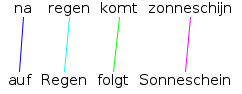
\includegraphics[scale=0.6]{Graphics/alignment.png}
\caption{A visualisation of a word alignment for the sentence pair (`Auf regen folgt sonneschein', `Na regen komt zonneschijn'). An arrow from source word $w_s$ to target word $w_t$ implies that $w_t$ was involved in the translation of $w_s$. This picture was created using the Alignment Visualiser developed by \cite{maillette2010visualizing}}
\label{fig:alignment}
\end{framed}
\end{figure}

\begin{definition}[Word-alignment]\label{def:alignment}
Given a source sentence $s = s_0 \cdots s_n$ and its translation $t = t_0 \cdots t_m$, an alignment is a set $a \subseteq \{0,1,\ldots,n\} \times \{0,1,\ldots,m\}$ such that $(x,y)\in a$ iff $s_x$ is translated into $t_y$.\footnote{In some definitions unaligned words are explicitly included in the alignment by adding an extra $NULL$ token to both source and target sets and including $(x,NULL)$ (or ($(NULL,y)$) in $a$ whenever word $x$ (or $y$) is unaligned. In our definition, unaligned words are not explicitly included: when a word $x$ is unaligned, this will be indicated by the absence of a word $y$ such that, respectively, $(x,y)$ or $(y,x)$, depending on whether $x$ was a source or target word.}
\end{definition}

Word alignments give rise to a straight-forward notion of translation equivalence: two sequences are translation equivalent if the words in the one sequence are translated only into words in the other sequence, and vice versa (both sequences are then called `translation admissible'). 

\subsection{Types of Word-Alignments}
\label{subsec:types_alignments}

There are several types of word-alignments, that describe different types of phenomena in translation. A summary of the restrictions corresponding to different kinds of alignments can be found in table \ref{table:alignments}. The example alignment depicted in Figure \ref{fig:alignment} is a very simple one. The alignment is one-to-one, as every word in both sentences is aligned to exactly one other word, and it is monotone, which means the order of source and target words is identical. A monotone one-to-one alignment indicates that no lexical or syntactical divergence complicated the translation.

\begin{table}
\footnotesize{
\begin{tabular}{|ll|}
\hline
one-to-one & $\forall x\forall y \big( (x,y)\in y \to \forall z \big( (z,y)\in a \to z=x \land (x,z) \in a \to z=y \big ) \big ) $\\
&\\
one-to many & $\forall x\forall y \big( (x,y)\in y \to \forall z \big( (z,y)\in a \to z= x \big) \big) $\\
&\\
many-to-one & $\forall x\forall y \big( (x,y)\in y \to \forall z \big( (x,z)\in a \to z=y \big) \big ) $\\
&\\
many-to-many & - \\
&\\
monotone & $\forall w \forall x\forall y \forall z \big ( \left ( (x,y)\in a \land (w,z)\in a \land x < w \right ) \to y < z \big )$\\
\hline
\end{tabular}
}
\caption{Different types of alignments and how they are characterised.}
\label{table:alignments}
\end{table}

In case of idiomatic translations, a one-to-one alignment does not suffice, as multiple source words are translated into multiple target words all at once. When aligning the English version of the saying in Figure \ref{fig:alignment} - `Every cloud has a silver lining' - to the Dutch sentence, it is not clear what should be aligned to what, if every word can have only one counterpart. Arguably, `has' should be aligned with `komt', as they are the only verbs in the sentence pair. However, when asking a bilingual Dutch and English speaker if `has' is a proper translation of `komt', the odds of obtaining an affirmative answer would be very slim. In this case, a more plausible alignment would align every Dutch word to every English word, indicating that the expression is translated as a whole. Such an alignment is called a phrasal alignment.

A similar adaptation is necessary when syntactic divergence occurs, although in such cases it is often unclear what the best alignment is. Consider, for instance, the word `does' in the sentence pair (`John does not live here', `John wohnt hier nicht'). As `does' has no clear translation in German, one might argue that it should be unaligned. However, the word seems to be connected with `live', so it could also be aligned with `wohnt'. A third option is to align `does' to `nicht', as it appeared with `not' when the sentence was negated \citep[example from][p.114]{koehn2008statistical}.



\subsection{Obtaining Word Alignments}

There are a few manually aligned corpora, but given the labour intensiveness of manually aligning corpora, they are mainly used to evaluate automatic aligners. We will briefly discuss manual alignments in \ref{subsubsec:man_alignments} after we have described how to generate alignments automatically.

\subsubsection{Automatic Word-alignments}

%FIND REFS ALIGNMENT IMPROVERS!! Maybe look in koehn
The reader may recall that word-alignments are established as a by-product of the word-based IBM models. Despite multiple efforts to improve on these techniques \citep[see][p.119-122 for some examples]{koehn2008statistical}, it is still common practice to use the alignments produced by the IBM tool GIZA++ \citep{koehn2007moses}. In the following 
paragraphs we will briefly explain how the IBM word-alignments are derived, and how many-to-many alignments can be constructed from them.

\paragraph{Expectation Maximization}
One step in the IBM models, is to learn a lexical translation model from a parallel corpus. This would be an easy task if word-alignments were directly visible from the data, as one could just count for each word how often it occurred in the text and how it was translated, and estimate a probability from these counts using relative frequency estimation. Conversely, the most probable word-alignments could be estimated if the lexical probability model was known. Learning word-alignments and lexical probabilities from a parallel corpus can thus be seen as a problem of incomplete data, that can be addressed with the expectation maximization (EM) algorithm \citep{dempster1977maximum}, which works as follows:\begin{enumerate}
\item Initialize the lexical probabilities (often with uniform distributions).
\item Compute the most probable alignment from the lexical probabilities (expectation).
\item Recompute the lexical probabilities from the alignment found in the previous step (maximization)
\item Iterate steps 2 and 3 until convergence.
\end{enumerate}

\noindent Note that the use of such an algorithm means that the larger the corpus is, the better the resulting alignments become. It is thus not possible to align just one sentence.

In IBM model 1 and 2, the models that describe how the alignments depend on the lexical probabilities are sufficiently simple to exhaustively run the EM algorithm, and a (global) optimum is thus guaranteed to be found. To find the most probable alignments in the higher IBM models, stochastic hill climbing is used. Excellent examples of complete executions of the algorithm for the different IBM models on very small toy corpora can be found in \cite[p88-113]{koehn2008statistical}.

\paragraph{Obtaining many-to-many alignments}
The IBM models consider the sequence of target words as being generated by the source words one by one. Therefore, although source words can be aligned to more target words, every target word is aligned to at most one source word and the resulting alignments are thus many-to-one. However, many-to-many alignments are often desired, as they match phenomena very common in practice. Alignments used to train SMT models on are often created by running the IBM models in both directions, and combining the resulting alignments. The three most common methods of merging two alignments $A_1$ and $A_2$ are:\begin{enumerate}
\item Union: $A_1\cup A_2$, containing all links from both alignments. The recall of the union will be high (as it contains many links), but as it contains all faulty alignment links from both alignments too, the precision is often quite low.\footnote{Given a set of desired alignment points $A_{gold}$, recall and precision of an alignment $A$ are defined as follows:\\
$$\text{Recall = }\frac{|A \cap A_{gold}|}{|A_{gold}|} \text{\hspace{10mm}Precision = }\frac{|A \cap A_{gold}|}{|A|}$$
Given the nature of $A_{gold}$, precision and recall are not the common metrics used to evaluate word alignments.}
\item Intersection: $A_1\cap A_2$, containing only the links that occur in both alignments. The resulting alignment is thus a one-to-one alignment. Contrary to the union, the intersection of $A_1$ and $A_2$ generally has a high precision, but a lower recall.
\item A more sophisticated method for combining alignments $A_1$ and $A_2$, is to first take the intersection, ending up with a selection of reliable alignment points, and then extend the alignment by adding neighbouring links and links $(i,j)$ for which holds that neither $e_i$ nor $e_j$ was aligned in the intersection \citep{och2000improved}, a heuristic. Pseudocode of this heuristic, called `grow-diag-final', can be found in \cite{koehn2008statistical}.
\end{enumerate}

%DIT MOET JE NOG INVULLEN!!!
Most current MT models that make use of alignments use the grow-diag-final method to obtain their alignments. The resulting alignments have a relatively high precision and recall \citep{och2000improved}, although they still contain several faulty alignment links. As mentioned before, several attempts to develop improved alignment models have been reported, where very different approaches have been explored. None of these methods has really found its way in the MT community. Besides the fact that it is hard to compare alignment methods across domains, it has been shown that improving alignment models does not necessarily result in better MT models \citep{indurkhya2010handbook}).

\subsubsection{Manual Word-alignments}\label{subsubsec:man_alignments}

As mentioned before, there are also a few manually aligned corpora. To address the issues raised in \ref{subsec:types_alignments}, manual alignments often distinguish between the alignment links that are sure, and those that are possible \citep{lambert2005guidelines}. The sure alignment links (indicated by the letter S) then represent unambiguous alignment links, while the possible alignment links (P) are less certain. Possible alignment links appear in case of phrasal translations, ambiguous translations, or in case two annotators disagree. 

All existing manually aligned corpora - the only ones known to the author of this thesis are presented in \cite{och2000improved}, \cite{graca2008building}, \cite{mihalcea2003evaluation}, \cite{pado2006optimal}, and \cite{ahrenberg2000evaluation} - are too small to train serious MT models on, and are mostly used to evaluate new alignment techniques (or sometimes for empirical analysis). A common metric used for this task is the alignment error rate (AER), which is defined as follows:

$$
\text{AER(S;P;A) = } - \frac{|\text{A}\cap\text{S}| + |\text{A}\cap\text{P}|}{|\text{A}| + |\text{S}|}
$$

A perfect score can thus be achieved by an alignment that has all the sure alignment points and some of the possible alignment points.



\subsection{Translation Equivalence through Word-alignments}

Translation equivalence can be defined in terms of word-alignments, as is described in Definition \ref{def:trans_eq}.

\begin{definition}[Translation Equivalence]\label{def:trans_eq}
If $(s,t)$ is a pair of source and target sentences and $A$ an alignment between $s$ and $t$, two sets of source and target words $w_s$ and $w_t$ are translation equivalent if and only if $$\forall x,y ( x\in w_s~(x,y)\in A \rightarrow y\in w_t \land x,y \in w_t~(y,x)\in A \rightarrow x\in A))$$
\end{definition}

The definition expresses the intuition that two sequences of words are translation equivalent if the words in the first sequence are translated only into words in the second sequence, and vice versa. This definition does not include a clause that states that such sequences need to be contiguous, a requirement that is often imposed when the translation parts are represented by nonterminal nodes in an SCFG.

\section{Compositional Translation Structures}
\label{sec:comp_structures}

Knowledge about translation equivalence of a translation pair restricts the set of structures according to which the one could have been translated compositionally into the other, as sequences that do not have a translation equivalent could not have been a part during the translation. In this section, we will define the set of structures according to which a sentence could have been compositionally translated, given its translation equivalent parts. As such trees are thus solely based on the alignment of the sentence, we will refer to such structures with the term  `alignment trees'.\footnote{This term is not new in this thesis, but is used by many authors in MT when referring to the hierarchical structures alignments give rise to.}

\subsection{Alignment Trees}
\label{subsec:alignment_trees}

For the purpose of devising alignment trees, the current definition of alignment is not particularly transparent. We will introduce, as far as this thesis goes, a change in notation for word-alignments, that is more suitable and clear for this purpose. The following two paragraphs will thus be a short recap of alignments and translation equivalence, but with a new notation. Figure \ref{fig:alignment2} is referred to as example dependency parse to clarify our new definitions.

\begin{figure}
\centering
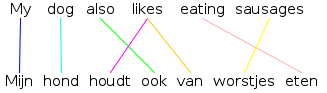
\includegraphics[scale=0.6]{Graphics/alignment1.png}
\caption{A one-to-many alignment of the English sentence `My dog also likes eating sausages.' and its translation `Mijn hond houdt ook van worstjes eten'. \citep[tool used to create picture: ][]{maillette2010visualizing}
}\label{fig:alignment2}
\end{figure}

\subsubsection{Set-permutations}
Following \cite{simaan2013hats}, we will represent an alignment by an ordered sequence of sets, of which the $n$th element specifies to which target word the $n$th source word maps. In case of a one-to-one alignment, this sequence is thus a permutation of the target word-positions, while in more complex alignments some of the target positions may appear multiple times in the sequence, or not at all. We will refer to such a sequence describing an alignment with the term `set-permutation', which is defined as follows:

\begin{definition}[Set-permutation]\label{def:sperm}
Given a source sentence $s = s_0 \cdots s_n$, its translation $t = t_0 \cdots t_m$, and an alignment $a$, let $a(i) = \{j~|~(i,j)\in a\}$ be the set with target positions that is linked to source position $i$. The set-permutation $\pi$ uniquely describing $a$ is defined as the ordered sequence of sets
$\langle a(0), \ldots, a(n) \rangle$.
\end{definition}

\noindent The set-permutation $\pi = \langle\pi_0, ..., \pi_n\rangle$ describing the alignment depicted in Figure \ref{fig:alignment2} would thus be $\langle \{0\}, \{1\}, \{3\}, \{2,4\}, \{6\}, \{5\}\rangle$. 

\subsubsection{Translation Equivalence for Set-permutations}

With the altered definition for alignments, a new definition for translation equivalence is required. In the following definitions, we will assume that $\bigcup_{i=0}^{n} \pi_i$ constitutes a contiguous sequence of numbers (thus there are no unaligned words). Although this is not always the case in practice, such a situation can always be achieved by only numbering the aligned target positions that are aligned, effectively switching the position numbers to the left whenever an unaligned word is found, and can thus be assumed without loss of generality.

\begin{definition}[Translation Admissibility]\label{def:transadd}
Let $\pi = \pi_1 \ldots \pi_n$ be a set-permutation describing a sentence pair $(s,t)$, a subset $\{\pi_i,\ldots,\pi_j\}$ is translation admissible if and only if for every integer $x \in (\pi_i\cup \ldots \cup\pi_j)$ holds that $x \notin (\pi_0\cup \ldots \cup \pi_{j-1} \cup \pi_{i+1}\cup\ldots\cup \pi_n)$.
\end{definition}

\noindent The notion of translation admissibility does not require contiguousness on either source or target side, which is desirable, as words are not necessarily translated into adjacent words in another language (for instance, in the running example `likes' translates into `houdt ...~van'). A projective tree representation of a compositional translation, however, demands that the non-terminal nodes cover contiguous subsequences in both source and target language, which leads to the following definition of non terminal translation part:

\begin{definition}[Non Terminal Translation Part]\label{def:transpart}
Let $\pi = \pi_1 \ldots \pi_n$ be a set-permutation describing a sentence pair $(s,t)$, a subset $\{\pi_i,\ldots,\pi_j\}$ is translation admissible if and only if $(\pi_i\cup \ldots \cup \pi_j)$ constitutes a contiguous range of integers (contiguousness on the target side), is a contiguous sequence in $\pi$ (contiguousness on the source side) and is translation admissible according to Definition \ref{def:transadd}.
\end{definition}

\noindent The alignment depicted in Figure \ref{fig:alignment2} thus has 5 non-terminal translation parts of length 1, 3 of length 2, 1 of length 3, 2 of length 4, 1 of length 5, and 1 of length 6 (see Figure \ref{fig:transequi}).

The number of translation parts in an alignment depends on the type of the alignment and is largest in case of a monotone alignment, that does not restrict the set of possible translation units at all. A completely monotone alignment of a sentence of $n$ words has $\frac{n\times n+1}{2}$ translation units. Note that unaligned words can cause exponential growth in the number of translation units.

\begin{figure}[!ht]
\begin{framed}
\small{
\begin{itemize}
\item \{0\} \hfill \{1\} \hfill \{3\} \hfill \{6\} \hfill \{5\} \hfill
\item \{\{0\},\{1\}\} \hfill  \{\{6\},\{5\}\} \hfill \{\{3\},\{2,4\}\}
\item \{\{1\},\{3\},\{2,4\}\}
\item \{\{0\},\{1\},\{3\},\{2,4\}\} \hfill \{\{3\},\{2,4\},\{6\},\{5\}\}
\item \{\{1\},\{3\},\{2,4\},\{6\},\{5\}\}
\item \{\{0\},\{1\},\{3\},\{2,4\},\{6\},\{5\}\}
\end{itemize}
}
\end{framed}
\caption{Translation units of alignment from \ref{fig:alignment2}}\label{fig:transequi}
\end{figure}

\subsubsection{Set-permutation Trees}

The set of alignment trees follows relatively straight-forwardly from the notion of parts: an alignment tree is a tree whose root dominates the entire sentence, and all of whose nodes correspond with translation equivalent units. To account for non-contiguous parts, nodes are allowed to expand in a combination of terminal and non-terminal nodes as well, provided that the terminals together constitute a translation admissible subset of the total sentence. An alignment tree will be defined in terms of allowed node expansions. If the top node of a tree covers the entire sentence, and all nodes are expanded as described in Definition \ref{def:exp1}, it recursively follows that all non-terminal nodes are translation parts and all leaf nodes together constitute a translation admissible subset, and the tree is thus a compositional translation tree for the corresponding sentence.

\begin{definition}[Expansion of a translation part]\label{def:exp1}
Let $\pi = \langle \pi_0, \ldots,\pi_n\rangle$ be a set-permutation that constitutes a part of a translation. An allowed expansion of $\pi$ into parts is described by a segmentation of $\pi$ as an ordered set of indices $B = \{j_0\negthinspace=\negthinspace 0, j_1, \ldots ,j_{m-1},j_m\negthinspace=\negthinspace n+1\}$ that segments $\pi$ into $m$ adjacent, non-overlapping and contiguous segments such that for all $~0\leq i < m$ holds that the subsequence $\pi_{j_i}\ldots\pi_{j_{i+1}-1}$ is a new non-terminal node that is a translation part, or $\pi_{j_i}\ldots\pi_{j_{i+1}-1}$ consists of a single word constituting a translation admissible unit with one or more other segments of $\pi$.
\end{definition}

Using Definition \ref{def:exp1}, a translation tree can be constructed top down, by recursively segmenting the entire sequence until only sequences of length 1 are left. Figure \ref{fig:alignment_tree} shows a possible alignment tree for the alignment from the running example: the sentence is firstly split into the two translation parts `my dog' and `also likes eating sausage', the former is then further split into two `my' and `dog', that also both constitute allowed translation parts. Also the right tree is further split up into translation parts, until the segmentation of `also likes' is reached, and no further division into allowed translation parts is possible. The phrase is therefore segmented into the non-terminal node covering part `also', and the leafnode covering the translation admissible word `likes'. Depending on its type, an alignment may have many different possible alignment trees. The current alignment has more than 40 different trees. The number of alignment trees can be exponential in the length of the sentence, if no restriction is placed on the branching factor of the nodes. Every alignment can be assigned at least one structure (the completely flat one).

\begin{figure}[!ht]
\centering
\Tree [.\{\{0\},\{1\},\{3\},\{2,4\},\{6\},\{5\}\} [.\{\{0\},\{1\}\} [.\{0\}  my ] [.\{1\} dog ] ] [.\{\{3\},\{2,4\},\{6\},\{5\}\} [.\{\{3\},\{2,4\}\} [.\{3\} also ] [.likes ] ] [.\{\{6\},\{5\}\} [.\{5\} eating ] [.\{6\} sausage ] ] ] ]
\caption{A possible alignment tree for the alignment of Figure \ref{fig:alignment} \label{fig:alignment_tree}}
\end{figure}

Note that the trees we have described are describing a compositional translation of the source side. The target side tree, however, can be constructed from this tree if it is known how the children of each node were reordered (this information is encoded in the set-permutation).


\section{Empirically Studying Compositionality}
\label{sec:empirical_studies}

We have showed that, given a word-alignment, it is always possible to construct a set of structures according to which a sentence could have been compositionally translated. Constructing such a set of structures, however, is not yet evidence for compositionality of translation. We do not know if the sentence was in fact translated as described by one of these structures, and whether this could have been predicted by a grammar. Investigating the set of alignment structures of sentences can be used to answer questions about the hypothetical underlying grammar that generated the data. Previously addressed questions can be roughly divided into two categories (we will later propose another perspective to these two categories):\begin{enumerate}%herformuleer dit nog een beetje
\item \textbf{Formal questions}. Several studies focus on the formal properties of the underlying grammar, asking questions as: `what is the minimal rank of the underlying grammar', or `how much of the corpus can be covered by a pure permutation'.
\item \textbf{Linguistic questions}. Other studies follow a different direction, starting out from monolingual syntax. In these studies, the focus lies on the explanatory power of monolingual syntax, and questions addressed include: `how many of the nodes of monolingual parse trees are translation equivalent according to an alignment', `if we stay true to monolingual parses, how far from bijective is the mapping between the non-terminal nodes'.
\end{enumerate}

In this section, we will discuss some previously conducted studies, and the answers they have found to these questions.

\subsection{Linguistic Questions}

Several studies focus on the explanatory power of transforming linguistic parse trees, hereby addressing the coherence between monolingual syntax and alignment trees. Even though they are run on different datasets, with different language pairs and use different criteria, they all find that linguistic parse trees do not coincide very well with translation corpora.

\subsubsection{Constituency grammars}

There are different ways of quantifying the suitability of monolingual linguistic parse trees. An often cited study is the one carried out in \cite{fox2002phrasal}. \citeauthor{fox2002phrasal} investigated how well linguistic phrases (i.e., constituents in a parse tree) stay preserved during translation from English to French. For her investigation, she used a manually aligned corpus created by \cite{och2000improved}, which contains 500 randomly selected sentences from the Canadian Hansard corpus. The manual alignments in this corpus are of type `sure' ($S$) and `possible' ($P$). Fox counted the number of times the translation of distinct syntactic constituents (on the English side) overlapped or `crossed'. We will not give a formal definition of a `crossing', but provide an example in Figure \ref{fig:fox}. Fox concluded that crossings - even after filtering out phrasal translations that necessarily result in crossings - are too prevalent to ignore (on average 2.854 per sentence if all alignment links are considered).\footnote{With a manual analysis of the crossings in the constituency parses she showed that many of them are not due to the lack of phrasal cohesion, but are caused by errors in the syntactic analysis or rewording and reordering in the translation. Her analysis, however, included only the crossings of the S alignment links - the ones on which all annotators agreed and that were not ambiguous - that constitute just a small part of the total set of crossings.}


\begin{figure}[!ht]
\centering
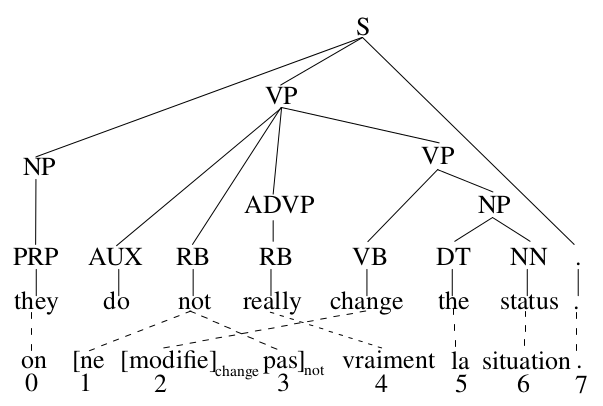
\includegraphics[scale=0.4]{Graphics/crossing.png}
\caption{An example of a crossing according to \cite{fox2002phrasal}.}\label{fig:fox}
\end{figure}

Her results are supported by others. \cite{galley2004s} generated constituency trees on the English side of the aforementioned Hansard corpus and tested how powerful a synchronous grammar should be to be consistent with the translation corpus. The power of the grammar was expressed in terms of the depth of the subtrees it generated, a standard CFG rule, that generates only single non-terminals, thus has depth 1. If rules of larger depth than 1 are needed, the non-terminal nodes of the syntactic source tree cannot be mapped bijectively to any target tree in a way consistent with the word-alignments. \citeauthor{galley2004s} found that only 19.4\% of the trees in the corpus could be covered entirely by one-depth-rules, and 85\% of the nodes (for the S alignments). Furthermore, he found that to cover the entire corpus with a grammar consistent with the allowed number of rule expansions should be no less than 17 for the S-alignments, and 23 for automatic alignments. For the English-Chinese corpus he analysed, the coverage of low-expansion rules was even lower: 16.5\% (of the trees) for rules with a single expansion, and 100\% only with a maximum of 43\% expansions per rule.

\cite{khalilov2012statistical} confirmed the inadequacy of child-reordering in work that focusses on source reordering preliminary to translation. Using LRscore \citep{birch2010lrscore} as a measure of success, they concluded that permuting the children of nodes in a constituency tree is insufficient to reach a perfect permutation of source-words in English-Dutch and English-Spanish translation data, even when deleting up to 5 layers of nodes in the parse tree is allowed.\footnote{Their score for English-Spanish, however, is surprisingly high: around 94.}


\subsubsection{Dependency Grammars}

Not very much literature focusses on the consistency of dependency grammars with translation data, but some articles can be found on the matter. In her study about crossings, \citeauthor{fox2002phrasal} also devoted a section on dependency grammars. She observed that dependency parses are more cohesive than constituency grammars, with
2.714 crossings per sentence, compared to 2.854 for constituency grammars. A study that focusses exclusively on dependency parses was presented in \cite{hwa2002evaluating}. She investigated how well predicate argument structures agree between English and Chinese, addressing the validity of the Direct Correspondence Assumption.\footnote{Which expresses the intuition that there exists a mapping between the syntactic relationships in two sentences that are each others translation, and is thus directly allied to compositional translation} \citeauthor{hwa2002evaluating} evaluated the quality of Chinese dependency parses that were projected directly from English to Chinese through a manual word-alignment. The resulting parses have a very low F-score (38.1), which is not surprising, as phrasal translations (multiple aligned words on source or target side) and unaligned target words always result in errors. \citeauthor{hwa2002evaluating} also observed this fact. They developed a small set of linguistically motivated rules, which boosted the F-score to 68.3, which is significantly higher, but still rather low. Also, it makes their work very specific, and hard to extend to other language pairs or contexts.

Another work along the same lines was presented by \cite{fung2006automatic}. \citeauthor{fung2006automatic} did not directly use dependency grammars, but learned cross-linguistic (English-Chinese) semantic verb frames. The learned argument mappings  had an accuracy of 89.3\%. It is unclear how their results compare to \citepos{hwa2002evaluating} results and dependency grammars in general, a fortiori because the exact nature of the learned semantic frames stays unclear.

\subsection{Formal Questions}

A second line of empirical research does not restrict source (or target) side trees to linguistic trees, but investigates the coverage of formal SCFGs. The majority of the empirical results on SCFGs focus on the coverage of binary trees \citep[e.g.,]{zhang2006synchronous,huang2009binarization}, or SCFGs in normal form \citep[e.g.,][]{sogaard2009empirical1,sogaard2009empirical2,sogaard2010can}. All concluded that the range of reordering phenomena occurring in real translation data are by far not as complicated as the worst case scenario sketched in \cite{satta2005some}.
%But also that...?

\cite{wellington2006empirical} seem to be the only onse who compared their results with linguistically restricted parse trees. On several dataset (covering translation from Chinese, Romanian, Hindi, Spanish and French to English), they found that maximally 5\% of the alignments could not be explained by a completely binary tree, while the failure rate for binary trees that were constrained by monolingual parse trees on the English side climbed to 15\% for French/English to 61\% for Chinese/English. The failure rate they found for non constrained binary trees is much lower than the one found by \cite{simaan2013hats}, who reported a coverage of 71.46\% for the manual alignments of the Hansard corpus for trees with a maximal branching factor of 2. The coverage of binary trees for automatic alignments was even lower: 52.84\%. This difference between the results of \cite{wellington2006empirical} and \cite{simaan2013hats} is most likely due to a different treatment of alignment links: the latter authors used all alignment links in the dataset, while the former treated many-to-one alignment links disjunctively, focussing on lower bounds. \cite{simaan2013hats} also reported the coverage of non binarisable (permutation) trees, which is surprisingly enough not much higher: 72.14\% and 56.56\% for manual and automatic alignments, respectively.


\section{Dependency Parses}
\label{sec:dep_parses}

The studies described in the previous section are conducted from two different perspectives, that we earlier described as linguistically oriented and formally oriented. The formally oriented studies take a bilingual perspective, starting from the data and trying to gain information about the system that generated it. The linguistically oriented studies start out from monolingual information about language, and try to assess its suitability as underlying system. Surprisingly enough, a study that combines the two perspectives, by trying to construct a bilingual grammar initially motivated by the data, but using monolingual information, does not really exist. In this thesis, we will try to narrow the gap between the two perspectives, by performing a study in which we combine bilingual information from a corpus and monolingual information from dependency parses. In this section, we will provide information about the background of dependency parses, and describe them formally. This section stands apart from the rest of this chapter, as it is not directly related to translation, but presents the last piece of background of the investigation conducted in this thesis.

\subsection{Background}

The dependency grammar is a cognitively motivated grammar formalism, that describes the perception of a sentence by the brain. Given its cognitive aim, dependency grammars are largely semantically motivated. Contrary to phrase structure grammars, that establish relations between constituents of a sentence, a dependency grammar does not divide a sentence up in phrases. Rather, it is based on the idea that in a sentence all words but one depend on another word in the sentence, via a(n asymmetric) binary relationship, that describes how the former word modifies or complements the latter. For instance, in the sentence `I really like writing my thesis', `my' depends on `thesis', as it complements it, and `really' depends on `like', which it modifies. Words can be said to have a valency, depending on how many dependents they need to be saturated (e.g., `like' would have a valency of two 2, as it needs both a subject and an object). The semantic background, combined with the fact that dependency grammars earlier showed to behave more coherent during translation than constituency grammars \citep{fox2002phrasal}, motivate a further investigation of this formalism. 

Although traditional dependency grammar (DG) has been used by linguists since the Middle Ages \citep{covington1990dependency}, modern DG is often seen as being created by \cite{tesniere1959elements}, whose cognitive motivation for it is worth citing:

\begin{quote}
The sentence is an organised whole; its constituent parts are the words. Every word that functions as part of a sentence is no longer isolated as in the dictionary: the mind perceives connections between the word and its neighbours; the totality of these connections forms the scaffolding of the sentence. The structural connections establish relations of dependency among the words. Each such connection in principle links a superior term and an inferior term. The superior term receives the name governor; the inferior term receives the name dependent. \citep[Translation:][]{ryan2013}
\end{quote}

The criteria for being a head-dependent pair are a mix of syntactic and semantic criteria \citep{nivre2005dependency}, and generally depend on the grammatical function the sentence or with respect to the word it depends on. Not all dependency grammars are identical in the relations they are considering, and their treatment of certain intuitively problematic constructions as coordination and conjunction \citep{nivre2005dependency}. In this thesis, we will follow the convention used in \cite{de2006generating}.

\subsection{Formally}

A dependency grammar is formally defined as follows \citep{hays1964dependency,gaifman1965dependency}:

\begin{definition}[Dependency Grammar]\label{def:depgram}
A dependency grammar is a quadruple $\langle R,L,C,F\rangle$, consisting of a set $L$ of terminal symbols (lexemes), a set $C$ of auxiliary symbols (lexical categories), a set $R$ of dependency rules over the auxiliary symbols $C$, and an assignment function $F : L\rightarrow C$.
\end{definition}

An example of a very simple (and unplausible) dependency grammar (according to which the dependency parse in Figure \ref{fig:depgraph} is grammatical) is shown in Figure \ref{fig:depgrammar}.

\begin{figure}[!ht]
\begin{framed}
$\mathcal{D} = \langle R,L,C,F\rangle$, where:\begin{enumerate}
\item[] $L$ = \{My, dog, also, likes, eating, sausage\}
\item[] $C$ = \{poss, nsubj, xvmod, xcomp, dobj, root\}
\item[] $R$ = \{(root, nsubj), (nsubj, poss), (root, xcomp), (xcomp, dobj), (root, xvmod)\}
\item[] $F = \left\{
  \begin{array}{l l l}
	F\text{(My)=poss} & \quad F\text{(dog)=nsubj} & \quad F\text{(also)=xvmod}\\
	F\text{(likes)=root}& \quad F\text{(eating)=xcomp} & \quad F\text{(sausage)=dobj} 
  \end{array} \right.$
\end{enumerate}
\end{framed}
\caption{A Toy Dependency Grammar}\label{fig:depgrammar}
\end{figure}


\noindent A dependency grammar prescribes dependency structures of sentences, that can be interpreted as graphs that satisfies the criteria that it is rooted and has only a single head (in other words, a dependency structure is a tree):

\begin{definition}[Dependency Graph]\label{def:depgraph}
A dependency graph of a sentence $s = w_1~\ldots~w_n$ is a directed acyclic graph $\mathcal{G} = \langle V, E\rangle$, in which $V = \{w_1, \ldots,w_n\}$ and $E$ is a set of edges such that $(w_i,w_j)\in E$ if and only if there is a dependency relation between $w_i$ and $w_j$. Furthermore, the graph satisfies the following two criteria:
\begin{enumerate}
\item $\exists\negthinspace w\in\negthinspace V$ s.t. $\forall w'\negthinspace\in\negthinspace V~(w,w')\negthinspace\notin\negthinspace E$ \hfill (rootedness)
\item $\forall w_1 w_2 w_3\negthinspace \in\negthinspace V\Big( (w_1,w_3)\negthinspace\in\negthinspace E~\land~(w_2,w_3)\negthinspace \in\negthinspace E\Big) \rightarrow w_1\negthinspace=\negthinspace w_2$ \hfill (single-headedness)
\end{enumerate}
The edges in $\mathcal{G}~$can be labeled with the function of the dependent.
\end{definition}

\noindent An example of a dependency graph is depicted in Figure \ref{fig:depgraph}. As the general definition of a graph is used, it is not immediately clear how  Definition \ref{def:depgraph} and Definition \ref{def:depgram} relate. To clarify: the set of vertices $V$ in $\mathcal{G}$ correspond to the lexical items, and thus the set $L$ in a dependency grammar. The edges $V$ correspond to the dependency relations $R$, while their labels must be in $C$. The function $F$ describes which functions words are allowed to have in the sentence. 

\begin{figure}[!ht]
\centering
\begin{dependency}[theme=simple]%[hide label]
\begin{deptext}[column sep=.5cm, row sep=.1ex]
%PRP\$ \& NN \& RB \&[.5cm] VBZ \& VBG \& NN \\
My \& dog \& also \& likes \& eating \& sausage \\
\end{deptext}
\deproot{4}{}
\depedge{2}{1}{poss}
\depedge{4}{2}{nsubj}
\depedge{4}{3}{xvmod}
\depedge{4}{5}{xcomp}
\depedge{5}{6}{dobj}
\end{dependency}
\caption{Dummy Dependency Graph, find other later}\label{fig:depgraph}
\end{figure}

A condition often put on dependency graphs, is projectivity, that prescribes a linear ordering of the nodes in the tree. Projectivity simplifies parsing, as it reduces the search space, but it is often argued that it deprives dependency grammar from its most important asset \citep{covington1990dependency,debusmann2000introduction}: the elegant method for handling discontinuous constituents (see Figure \ref{fig:npdeptree}). For fixed word order languages like English, in which phrases belonging together tend to stay together, projectivity is thus a reasonable criterion, but to account for languages in which there are less restrictions on the word-order (e.g., Russian, Latin) non-projectivity is often required to provide an intuitive analysis. An example of a non-projective in an otherwise fixed word-order language (Dutch) is depicted in Figure \ref{fig:npdeptree}.

\begin{figure}[!ht]
\centering
\begin{dependency}[theme=simple]%[hide label]
\begin{deptext}[column sep=.5cm, row sep=.1ex]
Ik \& weet \& dat \& hij \& me \& liet \& winnen\\
\tiny{I} \& \tiny{know} \& \tiny{that} \& \tiny{he} \& \tiny{me} \& \tiny{let} \& \tiny{win}\\
\end{deptext}
\deproot{2}{}
\depedge{2}{1}{}
\depedge{2}{6}{}
\depedge{6}{3}{}
\depedge{6}{4}{}
\depedge{6}{7}{}
\depedge{7}{5}{}
\end{dependency}
\caption{Non projective dependency graph of the Dutch sentence `Ik weet dat hij me liet winnen'.}\label{fig:npdeptree}
\end{figure}

\section{Summary}
\label{sec:summary}

In this chapter, we have discussed the difficulties of designing a system to compositionally translate natural languages. We have showed that there are several issues, and that it is hard to investigate their influence on the suitability of compositional translation as a strategy for translating natural language. We have argued that finding compositional solutions for specific parts of natural language for which a compositional treatment seems problematic will not provide us with a better understanding of the overall compositionality of translation, and neither will developing more translation models. We proposed to investigate the compositionality of translation through empirical analysis of real translation data, and laid the groundwork for such an analysis, by discussing how the compositionality of a corpus can be identified and investigated. We have discussed empirical studies related to the one conducted in this thesis, and we have pointed out that there seems to be a gap between the two perspectives they are taking. In the last section of the chapter we discussed dependency parses, that will be important for our own empirical analysis.